\chapter{Designmodell}

\section{GUI Externes Design}

\begin{figure}[H]
  \begin{center}
    {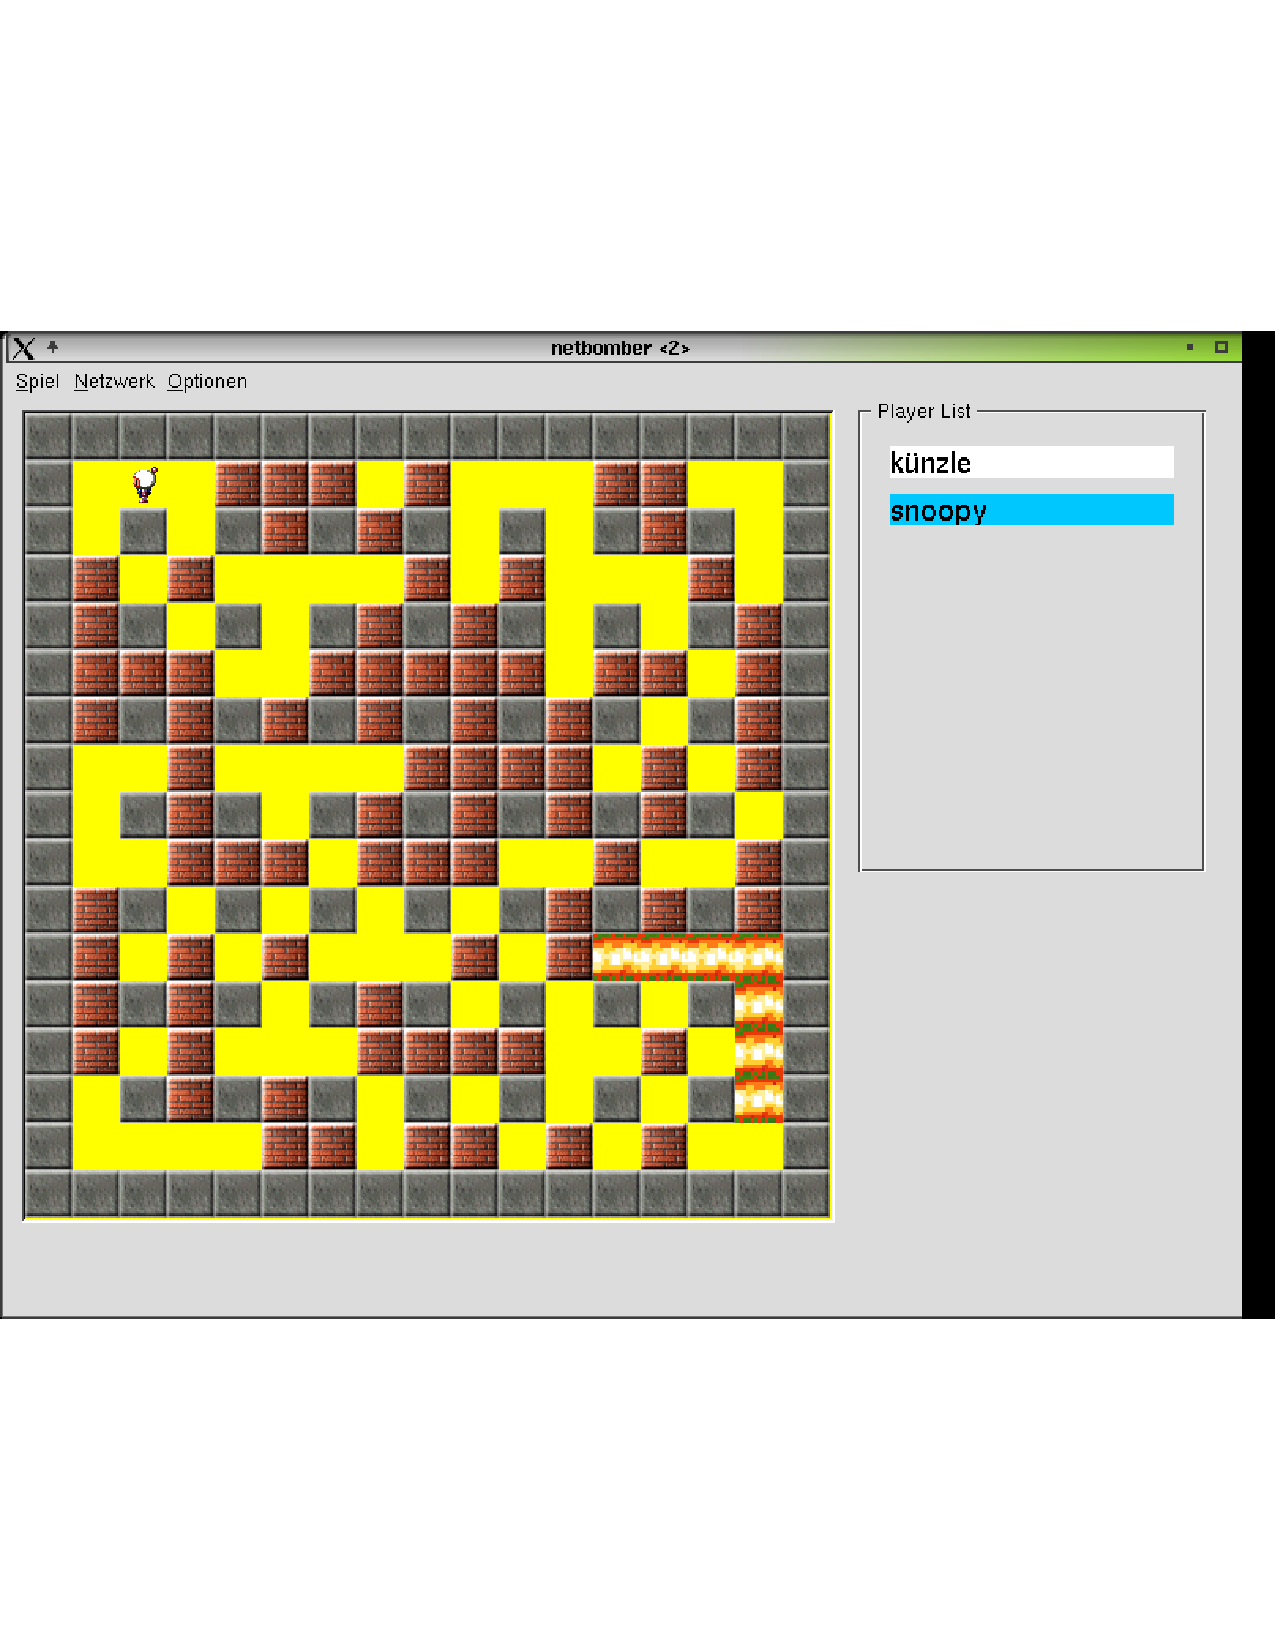
\includegraphics[height=12cm]{./images/spielfeld.pdf}}
  \end{center}
  \caption{Snapshot des GUIs}
\end{figure}

Wie aus dem Snapshot ersichtlich ist, ist das externe GUI Design
f"ur die Iteration 1 stark vereinfacht. Uns war wichtig, dass die
grundlegenden Funktionalit"aten (Spieler bewegen, collision detection)
einwandfrei funktionieren. Der Spieler kann "uber das Menu Spiel ein
neues Spiel starten oder die ganze Applikation beenden.
Mit den Pfeiltasten auf, ab, links und rechts steuert er die
Spielfigur.

\section{GUI Klassendiagramm}

\begin{figure}[H]
  \begin{center}
    {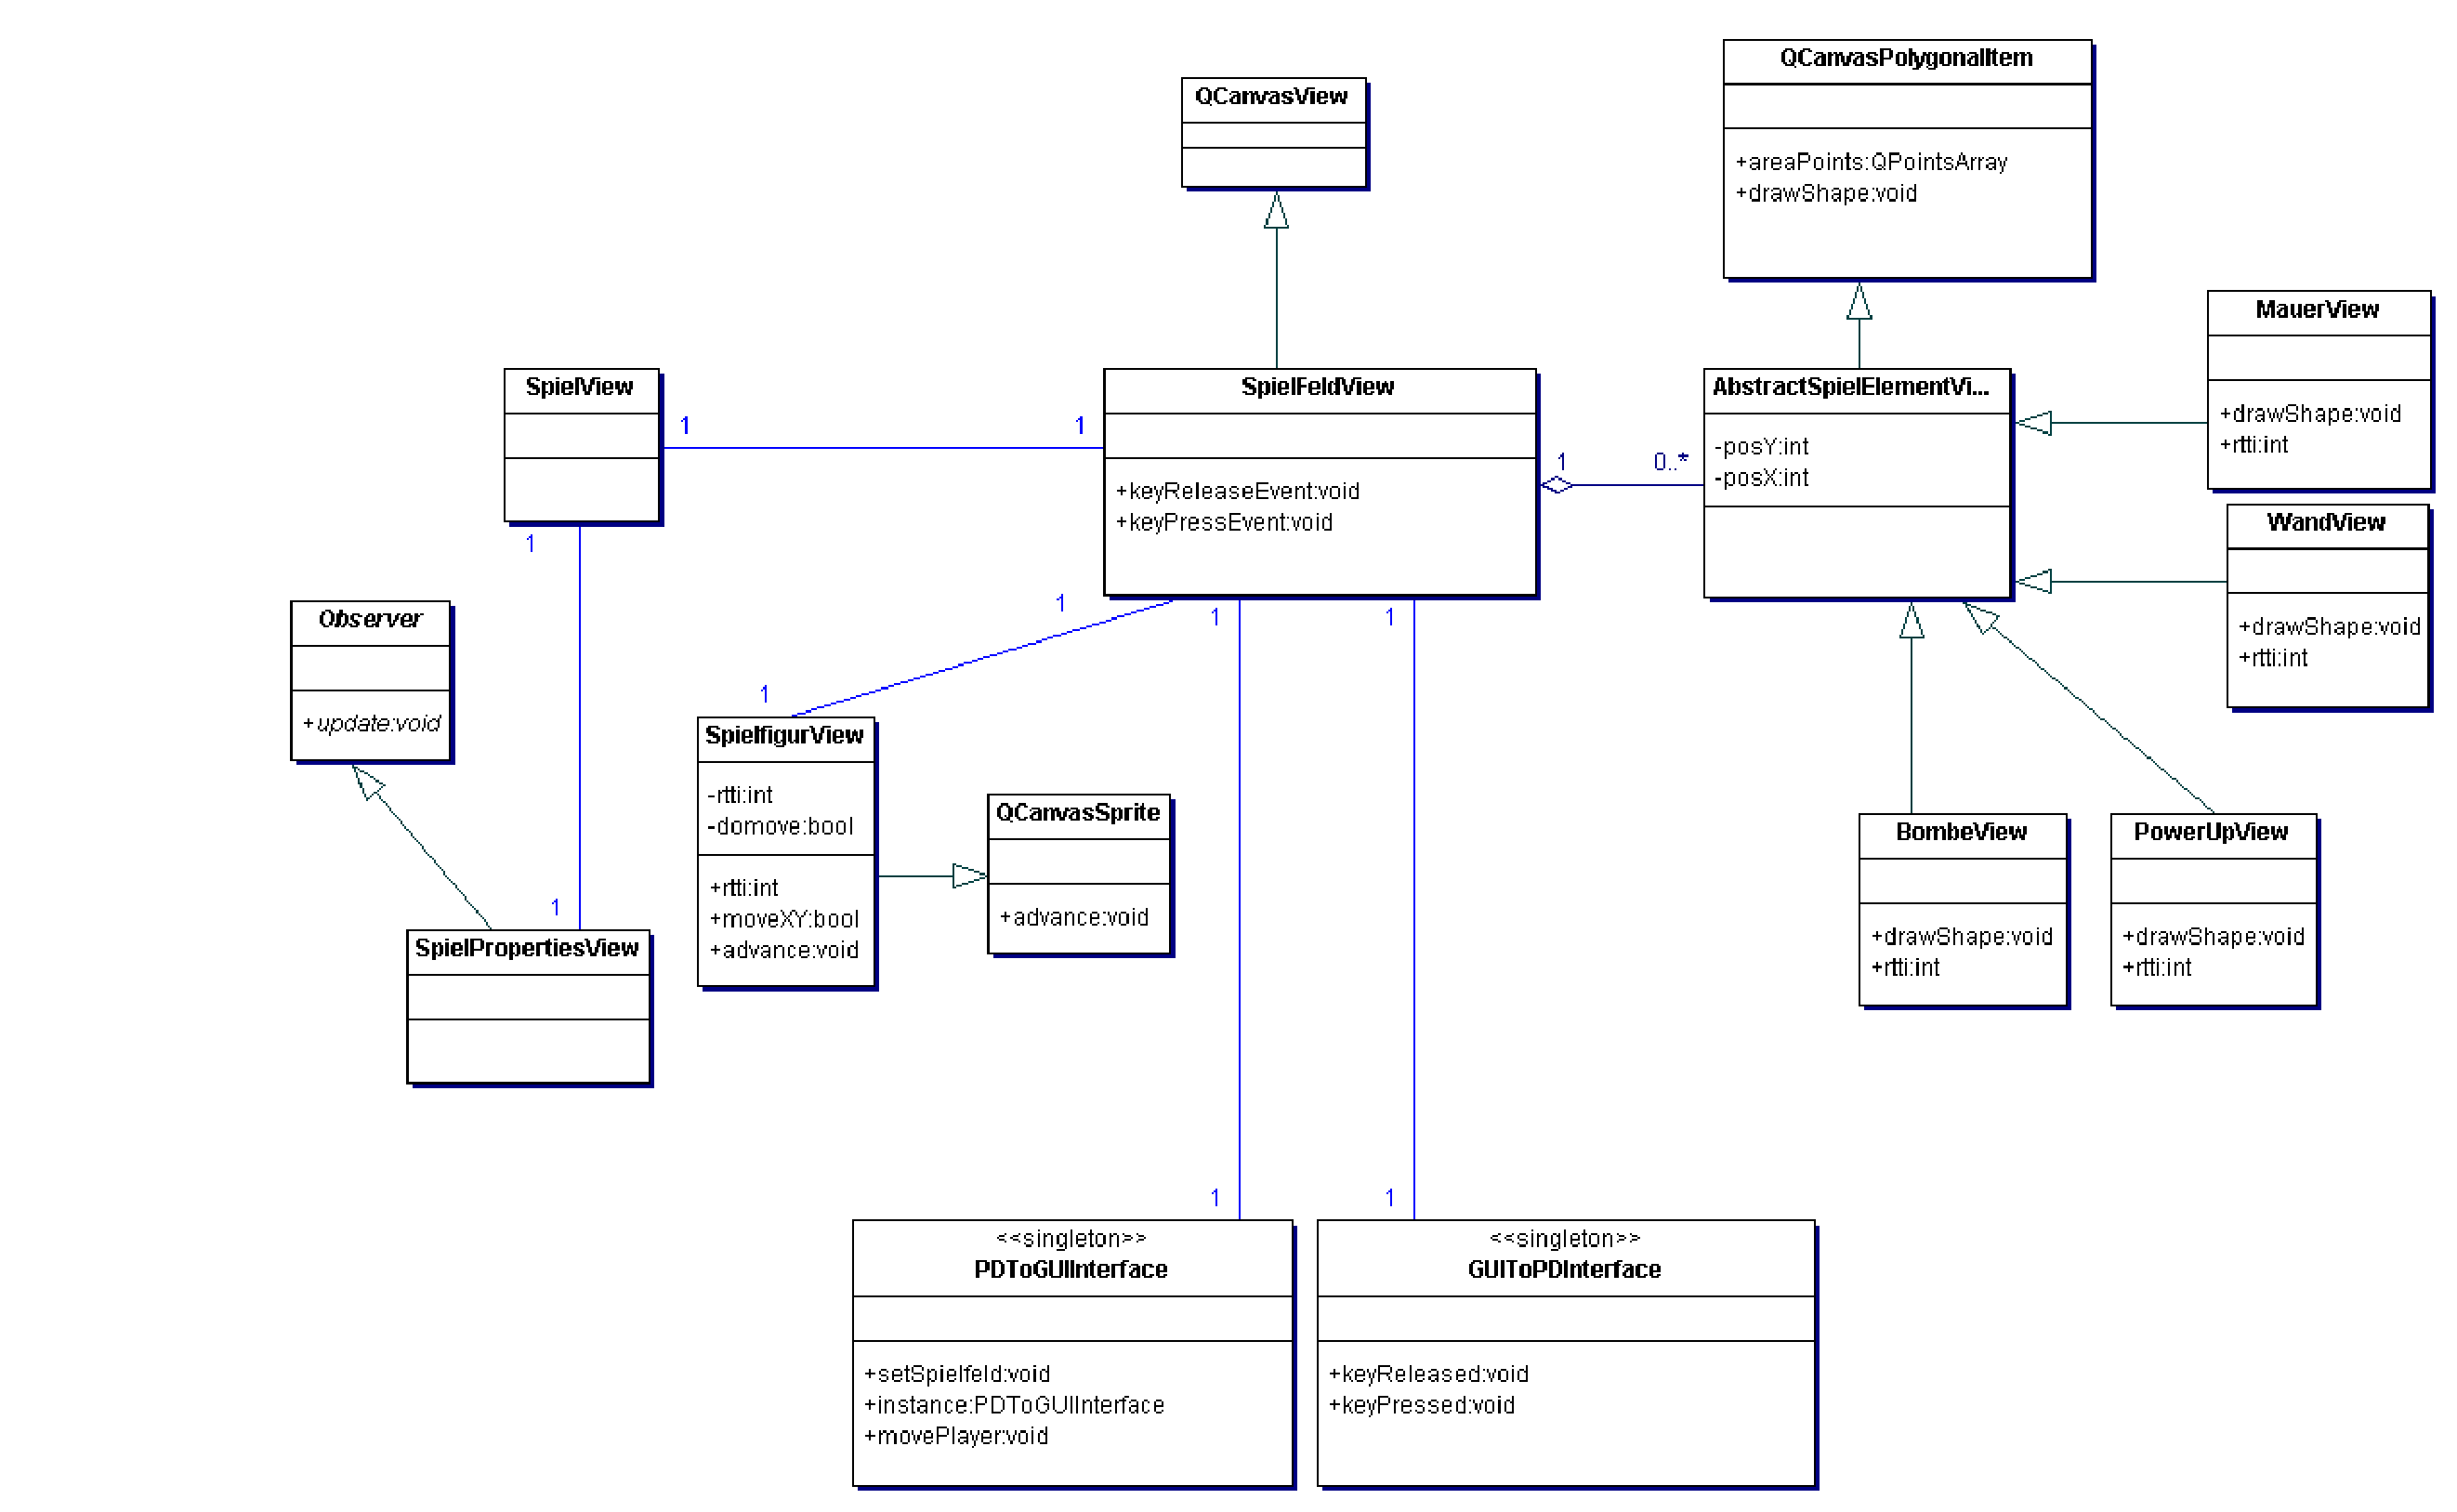
\includegraphics[height=10cm]{./images/guidesign.pdf}}
  \end{center}
  \caption{Klassendiagramm GUI}
\end{figure}

\section{GUI Sequenzdiagramme}

\begin{figure}[H]
  \begin{center}
    {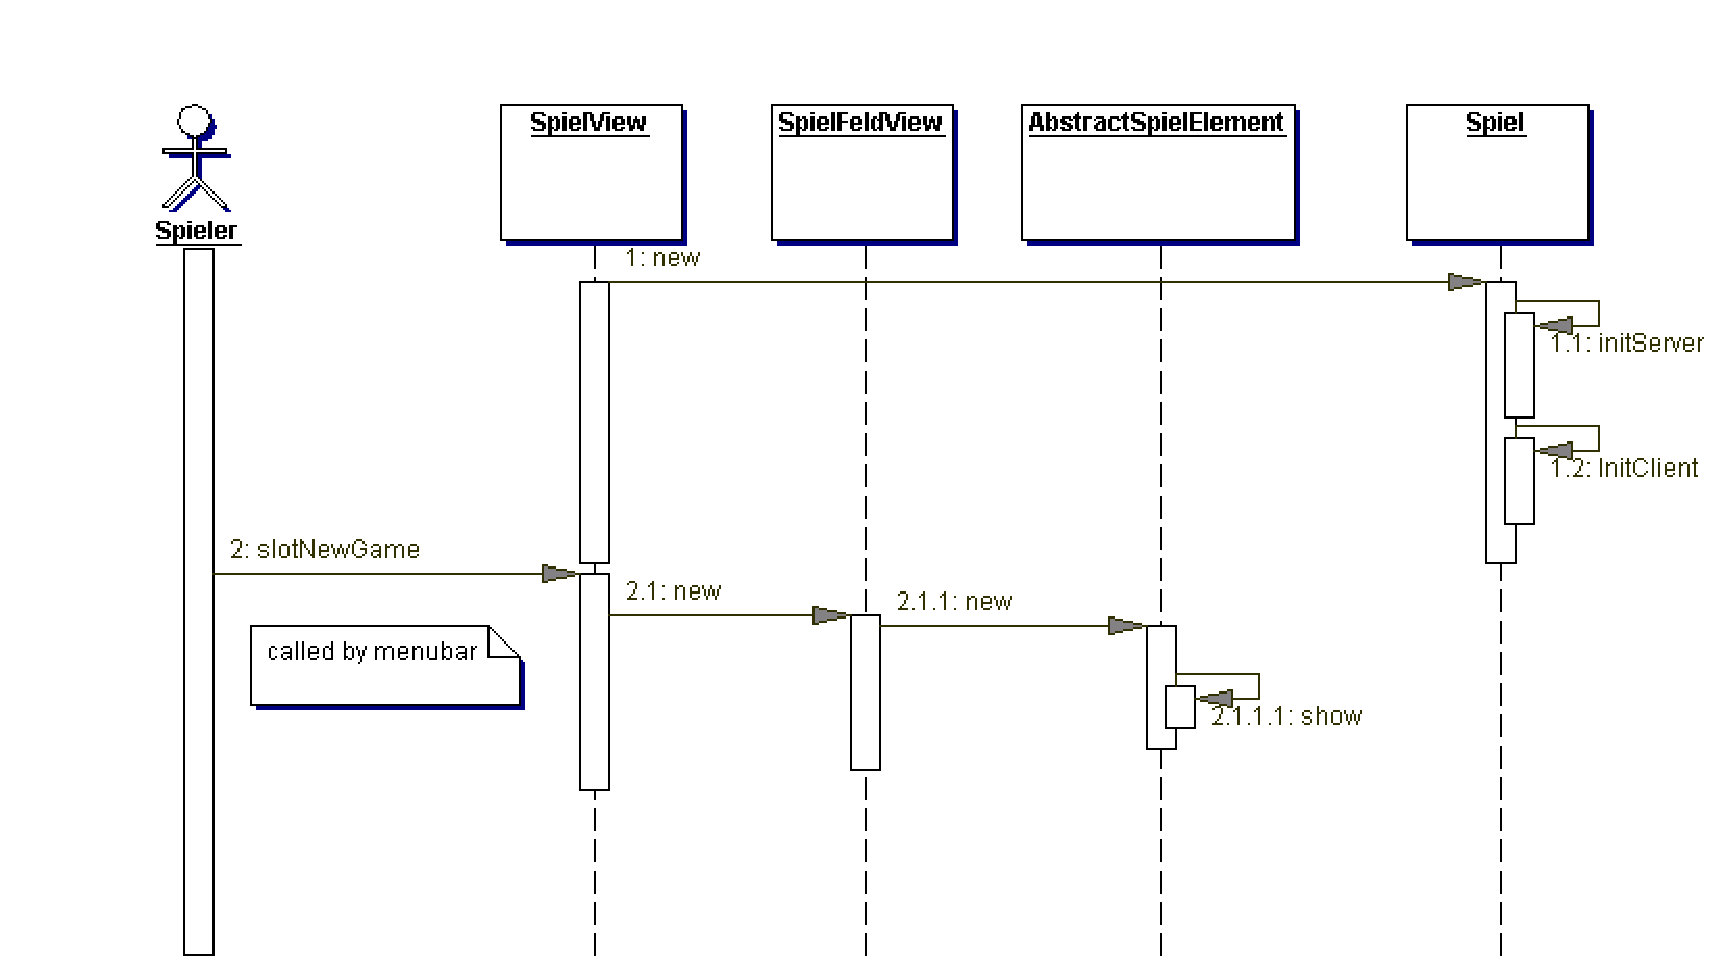
\includegraphics[height=6cm]{./images/neuesSpiel.pdf}}
  \end{center}
  \caption{Sequenzdiagramm f"ur neues Spiel}
\end{figure}

\section{GUI Klassenbeschreibung}

\subsection{Klasse SpielView}

Die Klasse SpielView enth"alt einzig allein ein Menu, welches
zum Starten eines neuen Spiels, zum Beenden des Spiels, oder
um das Optionsfenster zu "offnen, dient. Beim ersten Fall wird eine
neue Instanz der Klasse SpielFeldView erzeugt.

\subsection{Klasse SpielFeldView}

Sie ist sozusagen die Kernklasse im GUI Design. Diese Klasse verwaltet alle
sich auf dem Spielfeld befindenen Elementen (Aggregation zu AbstractSpielElementView).
Um das zu erreichen, wird sie von der Klasse QCanvasView abgeleitet. QCanvasView
ist die Pr"asentationsklasse f"ur QCanvasItems, also f"ur einzelne Grafikelementen. Auch das
Keyboard-Eventhandling erfolgt in dieser Klasse. Falls Keyboard-Events auftreten,
werden diese abgefangen, und nur die f"ur das Spiel relevanten Steuersignale werden
der Klasse PDToGUIInterface weitergeleitet, wo sie dann von der PD verarbeitet werden.
Gleichzeitig erh"alt sie von der Klasse GUIToPDInterface Methodenaufrufe, welche das Ver"andern
des UI's zur Folge haben (Verschieben der Spielfigur, entfernen / hinzuf"ugen von Mauern etc.).
Man kann sagen, die Klasse SpielFeldView ist v"ollig intelligenzlos,
sie nimmt nur Befehle von der Interfaceklasse entgegen, oder leitet an diese Steuersignale weiter.

\subsection{Klasse SpielfigurView}

Diese Klasse repr"asentiert die Spielfigur. Sie wird im Konstruktor der Klasse SpielFeldView
erzeugt. Ihre Koordinaten erh"alt sie ebenfalls von der Klasse SpielFeldView.

\subsection{Klasse AbstractSpielElementView}

Diese Klasse wurde von der Klasse QCanvasPolygonalItem abgeleitet. Sie erg"anzt diese
Klasse nur mit den Koordinaten. Gleichzeitig dient sie als Oberklasse f�r alle
auf dem Spielfeld befindenen Elementen, ausser der Spielfigur. Dies ist notwendig,
um die Aggregation zwischen SpielFeldView und AbstractSpielElement zu erreichen.

\subsection{Klasse MauerView}

Sie r"apresentiert auf dem Spielfeld eine unzerst"orbare Mauer. Das Attribut
rtti steht f"ur run time type information. Sie dient zur Identifikation.


%\section{PD Klassendiagramm}

%\begin{figure}[H]
%  \begin{center}
    %{\rotatebox{90}{\includegraphics[height=...cm]{./images/...}}}
%  \end{center}
%  \caption{Klassendiagramm PD}
%\end{figure}


\section{PD Klassendiagramm}

\begin{figure}[H]
  \begin{center}
    {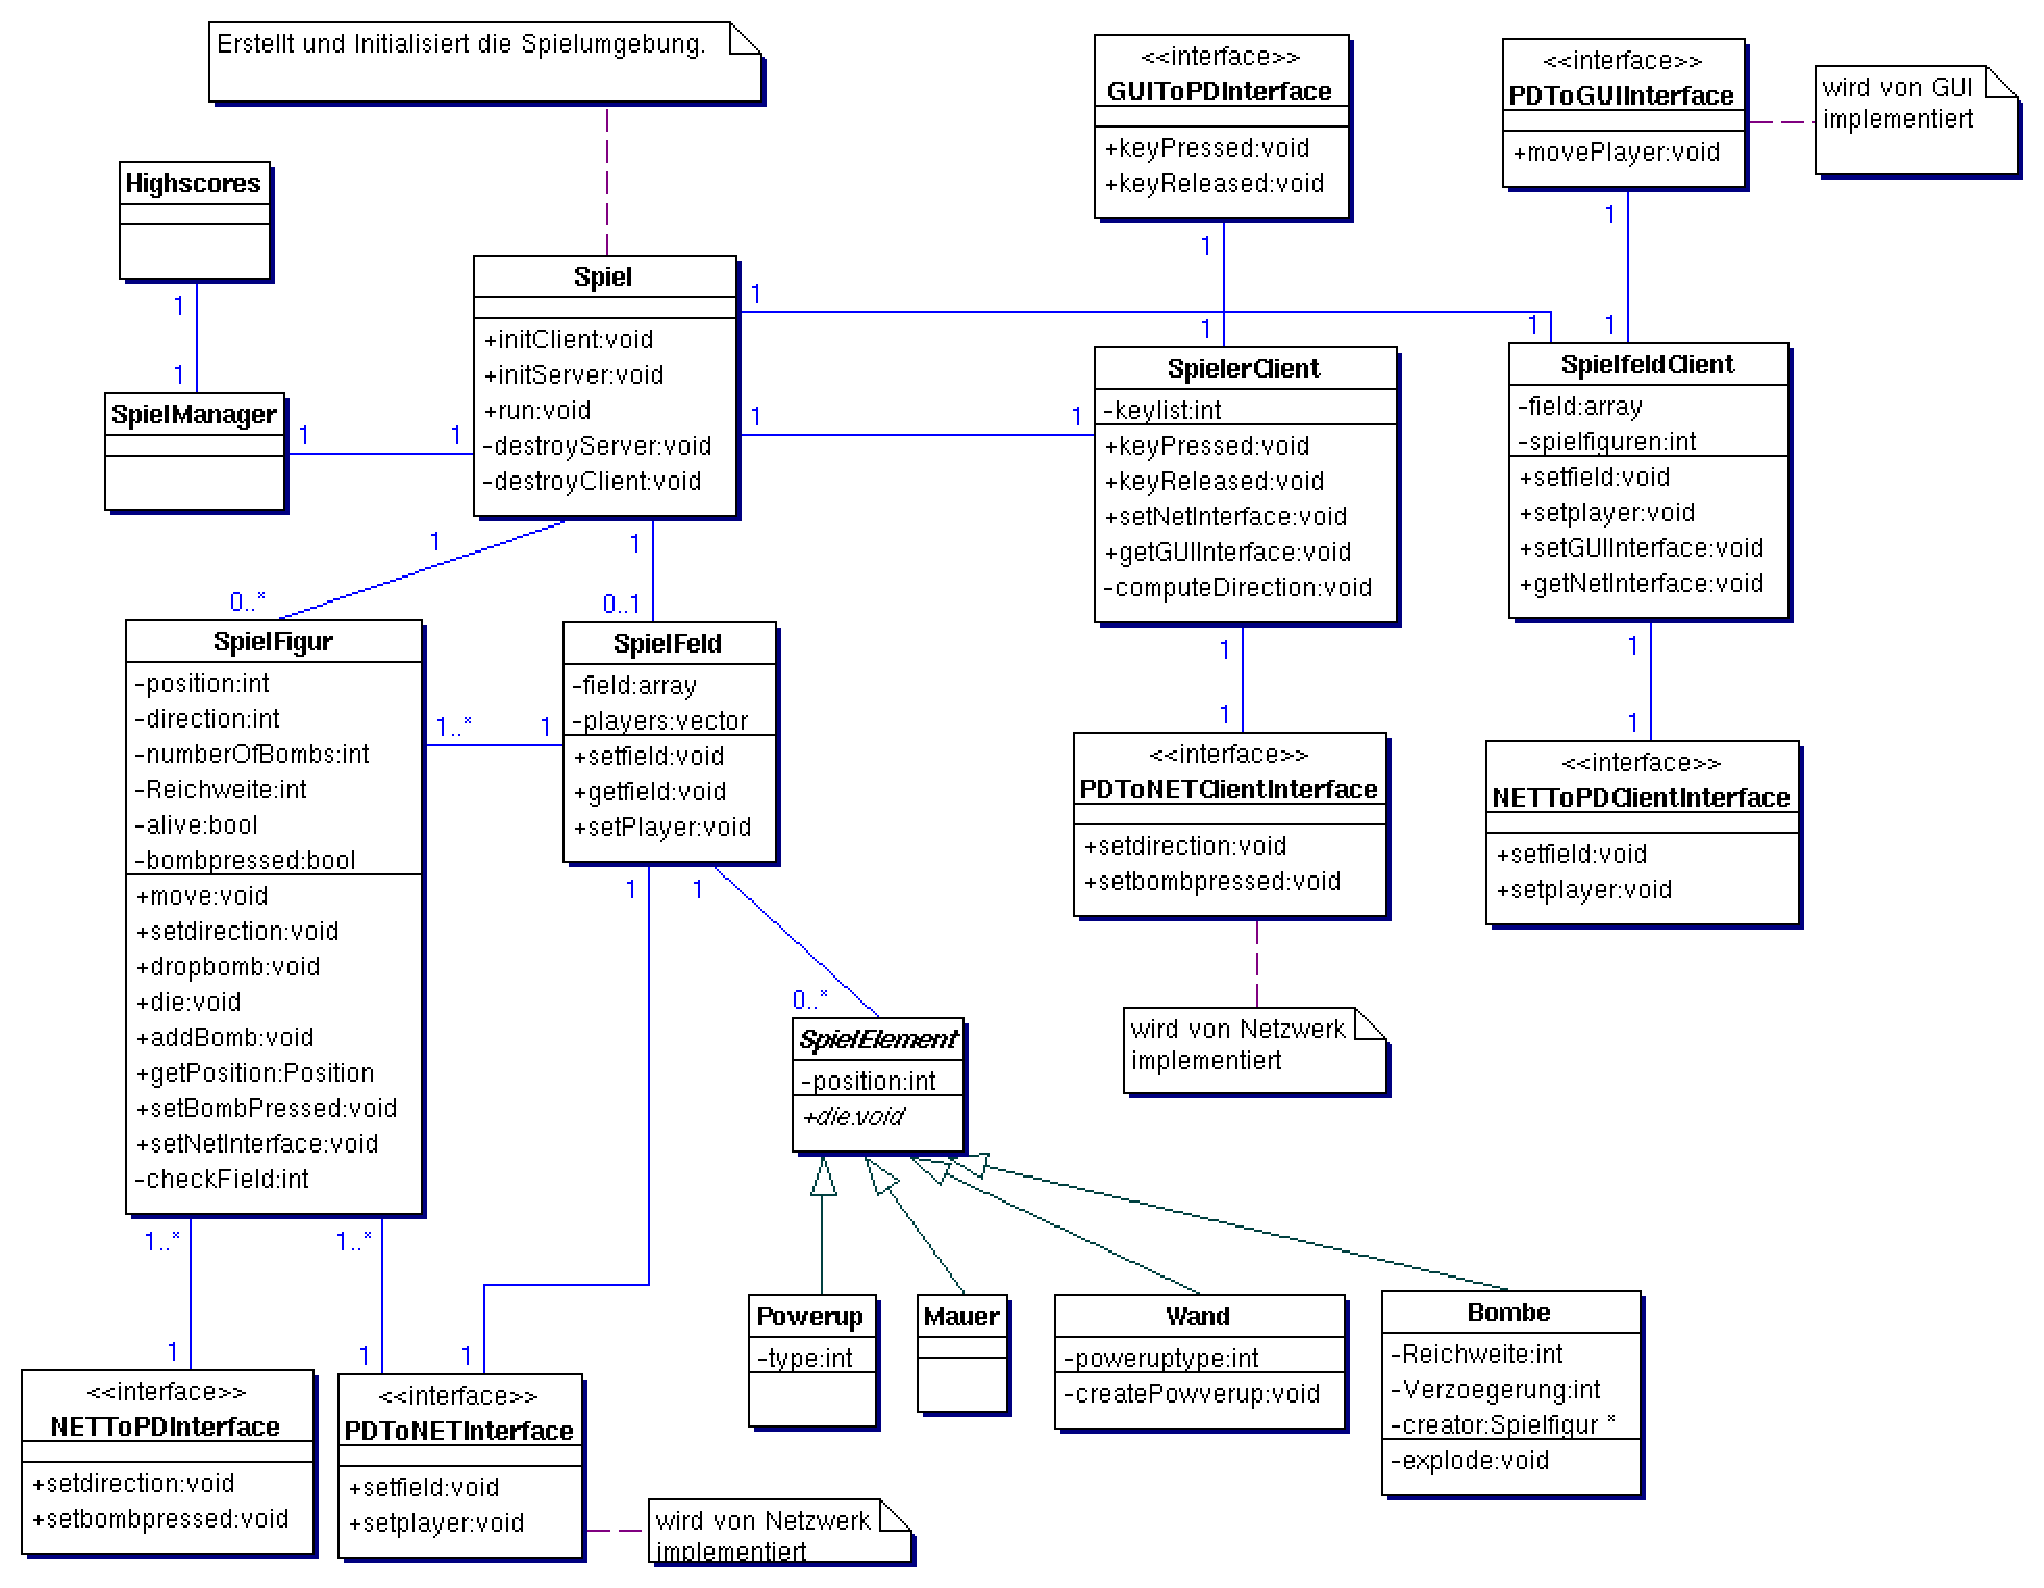
\includegraphics[height=10cm]{./images/pddesign.pdf}}
  \end{center}
  \caption{Klassendiagramm PD}
\end{figure}

\section{PD Sequenzdiagramme}

\begin{figure}[H]
  \begin{center}
    {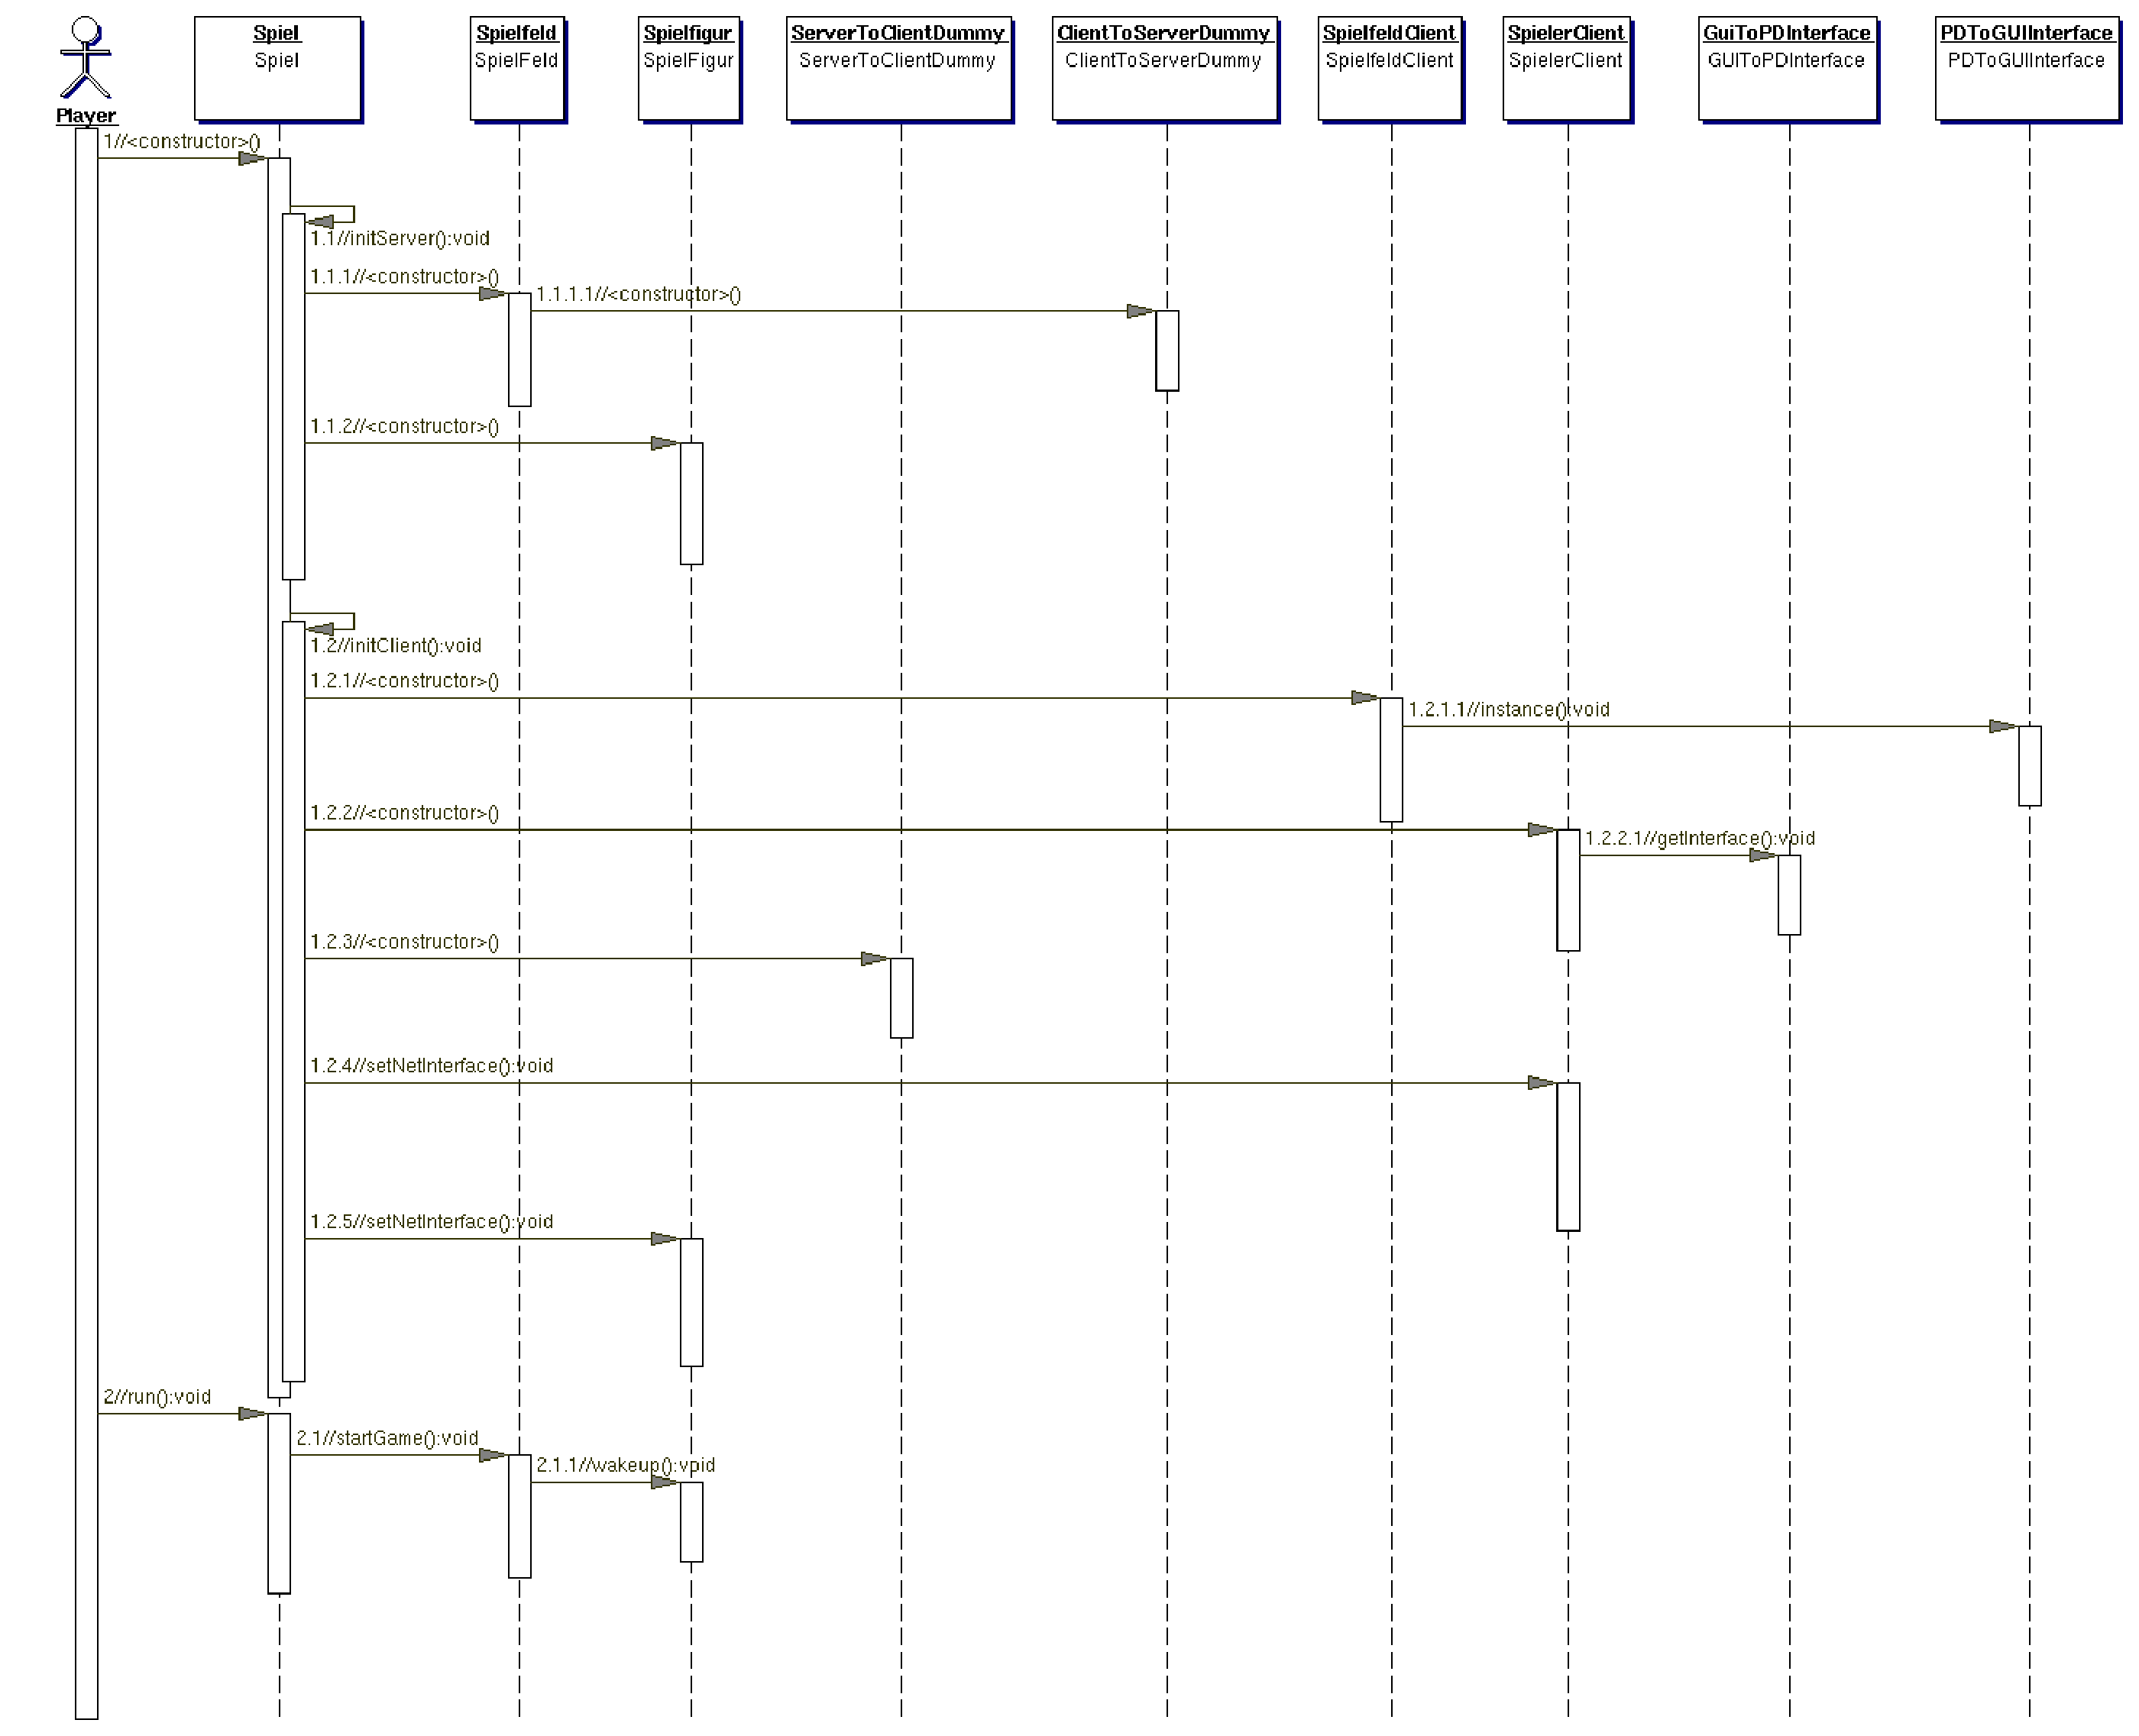
\includegraphics[height=10cm]{./images/startespiel.pdf}}
  \end{center}
  \caption{Sequenzdiagramm f"ur neues Spiel}
\end{figure}

% ProblemDomain  Klassenbeschrieb
% 19.4.2002 U.Heimann   Dokument erstellt
% 26.4.2002 U.Heimann   erweitert, korrigiert
%  2.5.2002 U.Heimann   �nderung Client/Server

\section{PD Klassenbeschreibung}
Die endg"ultige Version des Spiels soll "uber ein Netzwerk gespielt werden. Deshalb wird die PD in Server und Client unterteilt.
Die Klassen des Servers sind f"ur die Berechnung des gesammten Spielverlaufs (Positionen, Treffererkennung, ...) verantwortlich.
Der Client konvertiert die Steuerbefehle und schickt sie "ubers Netzwerk an den Server. Der Server berechnet die Auswirkungen
und schickt die "Anderungen zur"uck an alle Clients. Der Client reicht die "Anderungen wiederum an das User Interface weiter.
Jeder Spieler hat auf seinem Rechner eine Instanz des Clients, aber nur einer hat zus"atzlich noch eine Instanz des Servers.

\subsection{Klasse SpielManager}
Der Spielmanager sucht vor dem Spiel andere Spieler, die sich bei ihm anmelden k"onnen. Er startet (erzeugt) anschliessend das
Spiel mit den angemeldeten Spielern.

\subsection{Klasse Spiel}
Die Klasse Spiel erzeugt die restliche Spielstruktur (Spielfeld, Spielfiguren) je nach Anzahl
Spieler. Es wird immer ein Client erstellt, und beim Spielf"uhrer zus"atzlich noch ein Server. Sie ist daf"ur verantwortlich,
dass das Spiel mit allen Clients synchronisiert ist bevor das Spiel gestartet wird. \\
\subsubsection{Funktionen}
\begin{tabular}{p{50mm}p{90mm}}
+initClient()    : void  &  Initialisiert die Client-Umgebung. \\
+initServer()    : void  &  Initialisiert die Server-Umgebung. \\
+run()           : void  &  Synchronisiert und startet das Spiel. \\
-destroyClient() : void  &  R"aumt die Client-Umgebung nach Spielende auf. \\
-destroyServer() : void  &  R"aumt die Server-Umgebung nach Spielende auf. \\
\end{tabular}


\subsection{Klasse GUIToPDInterface (Singleton)}
"Uber diese Schnittstelle sendet das User Interface die Tastatureingaben des Spielers an die PD.\\
\subsubsection{Funktionen}
\begin{tabular}{p{50mm}p{90mm}}
+keyPressed(int key) : void    &  Taste key wurde gedr"uckt. \\
+keyReleased(int key) : void   &  Taste key wurde losgelassen. \\
\end{tabular}

\subsection{Klasse PDToGUIInterface (Singleton)}
"Uber diese Schnittstelle sendet die PD die "Anderungen des Spielfeldes an das User Interface.
(Diese Klasse wird vom GUI implementiert.) \\
\subsubsection{Funktionen}
\begin{tabular}{p{50mm}p{90mm}}
+movePlayer(int tox, int toy) : void  &  Die Spielfigur wird an die Koordinaten (tox,toy) verschoben. \\
\end{tabular}

\subsection{Klasse PDToNETInterface}
(vorl"aufig durch Netzwerk"uberbr"uckung ersetzt, bis Netzwerk implementiert ist)

\subsection{Klasse NETToPDInterface}
(vorl"aufig durch Netzwerk"uberbr"uckung ersetzt, bis Netzwerk implementiert ist)

\subsection{Klasse Spielfeld}
Die Klasse Spielfeld enth"allt ein Array das den aktuellen Zustand und die Positionen aller Spielelemente representiert. Sie hat
zugriff auf alle Spielentscheidenden Informationen. \\
\subsubsection{Attribute}
\begin{tabular}{p{50mm}p{90mm}}
-feld : array of Spielelement* &  Abbild des aktuellen Spielstandes. Jeder Eintrag im Array entspricht einem Feld. d.h. es k"onnen
                                  nicht mehrere Elemente auf einem Feld sein. (Spielfiguren werden hier nicht gespeichert!) \\
-playerlist : vector           &  Zeigerliste auf alle Spielfiguren des aktuellen Spiels. Die Position der Figur ist bei der Figur
                                  gespeichert.\\
\end{tabular}
\subsubsection{Funktionen}
\begin{tabular}{p{50mm}p{90mm}}
+setField(int x, int y, int item) : void  &  Setzt ein bestimmtes Element an die Koordinate (x,y). \\
+getField(int x, int y) : int item        &  Liefert das Element das sich an der Koordinate (x,y) befindet. \\
+setPlayer(Spielfigur* player) : void     &  Meldet einen neuen Spielfigur beim Spielfeld an. \\
\end{tabular}

\subsection{Klasse Spielfigur}
Die Klasse Spielfigur enth"allt alle wichtigen Informationen "uber Position und Zustand der Spielfigur. \\
\subsubsection{Attribute}
\begin{tabular}{p{50mm}p{90mm}}
-position : Position  &  Position der Spielfigur auf dem Spielfeld in (x,y) Koordinaten. \\
-direction : int      &  Richtung in die die Spielfigur gehen m"chte. (STAY, UP, DOWN, LEFT, RIGHT) \\
-numberOfBombs : int  &  Die Anzahl Bomben die er noch legen darf. -1 wenn Bombe gelegt wurde, +1 wenn seine Bombe explodiert ist
                         oder ein Bomben-Powerup aufgenommen wurde. \\
-reichweite : int     &  Reichweite der Bombe in Feldern. Wird der Bombe "ubergeben wenn sie gelegt wird. Wird erh"oht wenn ein
                         Flammen-Powerup aufgenommen wird. \\
-alive : bool         &  TRUE wenn die Spielfigur noch lebt. \\
-bombPressed : bool   &  TRUE wenn die Bomben-lege-Taste gedr"uckt ist. \\
\end{tabular}
\subsubsection{Funktionen} 
\begin{tabular}{p{50mm}p{90mm}}
+setDirection(int dir)     : void  &  Setzt die Laufrichtung der Spielfigur (STAY, UP, DOWN, LEFT, RIGHT). \\
+setBombPressed(bool bomb) : void  &  Setzt das bombPressd Flag (bomben-lege-Taste gedr"uckt). \\
+getPosition()  : Position pos     &  Liefert die aktuelle Position der Spielfigur. \\
+addBomb()                 : void  &  F"ugt eine Bombe zum Arsenal der Spielfigur hinzu. \\
+die()                     : void  &  Zerst"ort die Spielfigur wenn sie gesprengt wurde. \\
+setNetInterface(PD2NET*) : void  &  Setzt das Interface an das die "Anderungen der Position geschickt werden m"ussen. \\
-move()                    : void  &  Bewegt die Spielfigur um ein Feld in die aktuelle Richtung (direction). \\
-dropBomb()                : void  &  Legt eine Bombe an der aktuellen Position sofern noch Bomben im Arsenal. \\
-checkField()   : bool ok          &  Pr"uft ob ein Feld auf dem Spielfeld passierbar ist oder nicht. \\
\end{tabular}

\subsection{Klasse SpielerClient}
Die Klasse Spieler empf"angt die Benutzereingaben, bestimmt die daraus folgenden Aktionen und leitet sie an den Server weiter.\\
\subsubsection{Attribute}
\begin{tabular}{p{50mm}p{90mm}}
-keylist : array of bool  &  Speichert die Informationen welche Tasten momentan gedr"uckt sind und welche nicht. \\
\end{tabular}
\subsubsection{Funktionen}
\begin{tabular}{p{50mm}p{90mm}}
+keyPressed(int key) : void      &  Taste key wurde gedr"uckt. \\
+keyReleased(int key) : void     &  Taste key wurde losgelassen. \\
+setNetInterface(PD2NETI) : void &  Setzt das Interface an das die "Anderungen der Benutzereingaben geschickt werden m"ussen. \\
+getGUIInterface() : GUI2PD*     &  Liefert die Schnittstelle zur benutzereingabe. \\
-computeDirection() : void       &  Berechnet die Laufrichtung aus den Daten der keylist und sendet sie an den Server. \\
\end{tabular}

\subsection{Klasse SpielfeldClient}
Die Klasse SpielfeldClient hat ein vereinfachtes Abbild der Spielsituation gespeichert. Sie ben"otigt dieses sp"ater zur
berechnung der Explosionen. Sie empf"angt alle "Anderungen vom Server und gibt sie ans GUI weiter.\\
\subsubsection{Attribute}
\begin{tabular}{p{50mm}p{90mm}}
-field : array of int   &  Vereinfachtes Abbild der Spielsituation. \\
-players : array of Pos &  Die Positionen der Spieler auf dem Spielfeld. \\
\end{tabular}
\subsubsection{Funktionen}
\begin{tabular}{p{50mm}p{90mm}}
+setField(int x, int y, int item) : void  &  Setzt ein bestimmtes Element an die Koordinate (x,y). \\
+setPlayer(int x, int y, int nr)  : void  &  Setzt die Spielfigur (nr) an die Position (x,y). \\
+getNetInterface() : NET2PD*     &  Liefert das Interface auf das die "Anderungen auf dem Spielfeld geschickt werden m"ussen. \\
+setGUIInterface(PD2GUI*) : void &  Setzt die Schnittstelle zur Spielfeldanzeige. \\
\end{tabular}

\subsection{Klasse SpielElement}
Abstrakte Klasse von der alle Objekte abgeleitet sind die auf dem Spielfeld platziert werden k"onnen. (ausgenommen Spielfiguren) \\
(Spielelement werden im 1. Prototyp noch nicht eingesetzt.)
% Ende ProblemDomain Klassenbeschrieb

